\documentclass{llncs}

\usepackage{xcolor}
\usepackage{amssymb} 
\usepackage{tikz}
\usepackage[autostyle]{csquotes}

\usetikzlibrary{positioning}
\usetikzlibrary{arrows,automata}

\title{Handling String-number Conversion in String Constraint Solving}
\author{}
\institute{}


%%%%%%%%%%%%%%%%%%%%%%%%%%%%%%%%%%%%%%%%%%%%%%%%%%%%%%%%%%%%%%%%%%%%%%%%%%%%%%
\begin{document}
%%%%%%%%%%%%%%%%%%%%%%%%%%%%%%%%%%%%%%%%%%%%%%%%%%%%%%%%%%%%%%%%%%%%%%%%%%%%%%
\newcommand{\hide}[1]{}

\newcommand{\todo}[1]{{\color{blue}TODO: #1}}
\newcommand{\sti}[1]{\mbox{\textbf{toInt}($#1$)}}
\newcommand{\its}[1]{\mbox{\textbf{toStr}($#1$)}}
\newcommand{\varn}{\mbox{$\mathbb{V}_n$}}
\newcommand{\vars}{\mbox{$\mathbb{V}_s$}}
\newcommand{\cvar}{\mbox{$\mathbb{X}$}}
\newcommand{\modelof}[1]{[\![#1]\!]}
\newcommand{\true}{\mbox{$\mathsf{true}$}}


\newcommand{\enc}[1]{Enc(#1)}
\newcommand{\ch}[1]{\mbox{`#1'}}
\maketitle


%%%%%%%%%%%%%%%%%%%%%%%%%%%%%%%%%%%%%%%%%%%%%%%%%%%%%%%%%%%%%%%%%%%%%%%%%%%%%%
\section{Introduction} \label{section:introduction}
%%%%%%%%%%%%%%%%%%%%%%%%%%%%%%%%%%%%%%%%%%%%%%%%%%%%%%%%%%%%%%%%%%%%%%%%%%%%%%

\todo{Why this problem is important? Need to say it is used often, e.g., read 
from text file or user input. Why this problem is challenging? It is undecidable. Some tricky cases 
using string as array index. Bounded SAT-based encoding might not work even for 
very simple constraints. e.g., $y=str2int(x) \wedge y>9999999$, if $x$ is a 
ASCII string, then XXX boolean variables are required. Or we can just propose 
an example that all major solver fails. Maybe we still say our approach is still over-approximation + under-approximation, in this case, need to think how to present the over-approximation part. Maybe no CEGAR is fine.}


In this paper, we propose an approach that handles string constraints with string-number conversion efficiently. The approach combines techniques from both automata theory and SMT solving to explore the model space of a string constraint systematically. More specifically, instead of allowing the variable domain to be arbitrary strings from a finite alphabet, we restrict the search space of each string variable to strings that obey some predefined and parameterized pattern. By adjusting the parameters, one can easily enlarge or prune out the potential solution space. In paper, we propose to use patterns defined by \emph{symbolic flat automata}, the automata are very expressive yet allows very efficiently manipulation. For example, it avoids the alphabet 
explosion problem that the approach in~\cite{PLDI2017} suffers.


Based on the symbolic flat automata encoding, we manage to convert the 
string-number function to a constraint consisting of both 
polynomials and exponentials. To the best of our knowledge, the satisfiability 
problem of a mix of polynomials and exponentials is still open. For the 
particular case with only one number variable exponent, the satisfiability can 
be decided using the algorithm in~\cite{POPL2019}. However, the algorithm involves a quantifier elimination procedure, which is double-exponential to the length of the input formula and hence is not scalable to large instances.  \todo{check correctness of the above statement} For bounded numbers, our approach converts string-number function to a linear integer constraint.
To ease presentation, in the main text, we only consider string constraints consisting of \emph{equality constraints (a.k.a. word equation)}, \emph{length constraints}, and \emph{string-number conversion} functions. We describe the extension to support transducer and membership constraints in the appendix. 


\hide{
suggest restricting the string domain to $0^*[0-9]^k$, where $k$ is the maximum 
digit allowed in the corresponding number value. In programming languages 
such  as JavaScript or Python, a number with $k$ digits can be converted from a 
string of length arbitrarily longer than $k$. For example, $12 = 
str2int(``0000012")$. That is why we use $0^*$ at the beginning of the pattern.
Under this domain, we can convert the string-number conversion constraints to 
linear integer constraints, which is much easier to solve. In our experience, 
usually, it suffices to find a solution using a small $k$ for a satisfiable 
constraint. Note that a 64-bit integer number corresponds to a string with 
$k\leq 21$.}







%%%%%%%%%%%%%%%%%%%%%%%%%%%%%%%%%%%%%%%%%%%%%%%%%%%%%%%%%%%%%%%%%%%%%%%%%%%%%%
\section{Preliminary} \label{section:preliminary}
%%%%%%%%%%%%%%%%%%%%%%%%%%%%%%%%%%%%%%%%%%%%%%%%%%%%%%%%%%%%%%%%%%%%%%%%%%%%%%
We use $\mathbb{N}$ and $\mathbb{Z}$ to denote the sets of natural numbers and 
integers. For a set $A$, we use $|A|$ to denote its size. For a string $w$, we 
use $|w|$ to denote its length. We $\epsilon$ to denote an empty string and use $w_1\cdot w_2$ to denote the concatenation of strings $w_1$ and $w_2$. Let $S$ be a finite set of symbols. We use $S^+$ to denote the set of string over $S$ and $S^* = S^+\cup \{\epsilon\}$. We define $S_\epsilon =S\cup\{\epsilon\}$. A language 
$L$ over $S$ is a set of strings in $S^*$. 


%%%%%%%%%%%%%%%%%%%%%%%%%%%%%%%%%%%%%%%%%%%%%%%%%%%%%%%%%%%%%%%%%%%%%%%%%%%%%%
\section{String Constraints} \label{section:sc}
%%%%%%%%%%%%%%%%%%%%%%%%%%%%%%%%%%%%%%%%%%%%%%%%%%%%%%%%%%%%%%%%%%%%%%%%%%%%%%
Fix a finite alphabet $\Sigma \subseteq \mathbb{N}$, a finite set of string variables $\vars$ ranging over $\Sigma^*$, and a finite set of natural number variables $\varn$. Note that here we assume the alphabet is a finite subset of natural numbers. Essentially, we try to capture the numerical encoding of symbols (e.g., in ASCII, `A' is encoded as $65$) in computers. We write $[n,m]$ for the set of numbers (or symbols in $\Sigma$) $\{k\mid n\leq k \leq m\}$. A \emph{term} is an element in $(\vars\cup \Sigma)^*$. An \emph{interpretation} is a mapping from $\vars\cup \varn$ to $\Sigma^* \cup \mathbb{N}$. We lift 
it to terms by defining $I: (\vars\cup \Sigma)^* \rightarrow \Sigma^*$ with $I(a) =a$ for $a\in \Sigma$ and $I(t_1 \cdot t_2) = I(t_1)\cdot I(t_2)$. 

The \emph{string-number conversion function} $\sti{x}$ is defined as follows. For $x\in [0,9]^+$ and $a\in [0,9]$, we have $\sti{a}=a$ and $\sti{x\cdot a} = 10\times \sti{x}+a$. For $x\notin [0,9]^+$, $\sti{x}=-1$. 

For a number $n=a_n*10^n+a_{n-1}*10^{n-1}+\ldots+a_0$ for $a_i\in [0,9], i\in [0,n]$, the \emph{number-string conversion function} $\its{n}=a_ia_{i-1}\ldots a_0$~\footnote{Notice that only positive integer is supported in this semantics. This is the semantics used by most of the SMT solvers, and hence we follow it in this paper. This is not a restriction, since conversing from negative integer can still be encoded using the positive only version.}.

A \emph{equality constraint} $\phi$ is of the form $t_1 = t_2$ where $t_1, 
t_2$ are terms in $(\vars\cup \Sigma)^*$. The \emph{model} of $\phi$ is the set of interpretations $\modelof{\phi}=\{I\mid 
I(t_1)=I(t_2)\}$. A \emph{disequality constraint} is of the form $t_1 \neq 
t_2$ and is interpreted analogously.

An \emph{integer constraint} $\phi$ is a linear constraint over the variables in $\varn$, numerical values of strings $\sti{x}$, and length of a string $|x|$, for all string variables $x$ in $\vars$.
%Formally, assume that $\vars=\{x_i,\ldots,x_n\}$ and $\varn=\{y_i,\ldots,y_m\}$, a length constraint is of the form $(\sum_{i\in[1,n]}(j_i \times \sti{x_i}+k_i\times |x_i|)+ \sum_{i\in[1,m]}(l_i \times y_i)) \odot k$, where $\odot \in \{>,\geq, =, \leq, <\}$, and $j_i,k_i,l_i,k\in \mathbb{Z}$. We define $\modelof{\phi}= \{I \mid (\sum_{i\in[1,n]}(j_i \times \sti{I(x_i)}+k_i\times |I(x_i)|)+ \sum_{i\in[1,m]}(l_i \times I(y_i))) \odot k \}$.
We define  $\modelof{\phi}= \{I \mid I(\phi)= \true \}$.

%%%%%%%%%%%%%%%%%%%%%%%%%%%%%%%%%%%%%%%%%%%%%%%%%%%%%%%%%%%%%%%%%%%%%%%%%%%%%%
\section{Symbolic Flat Automata} \label{section:sfa}
%%%%%%%%%%%%%%%%%%%%%%%%%%%%%%%%%%%%%%%%%%%%%%%%%%%%%%%%%%%%%%%%%%%%%%%%%%%%%%
A \emph{finite-state automaton} (FA) is a tuple $(Q,T,\Sigma,q_0,q_m)$, where $Q$ is the set of states, $T\subseteq Q\times \Sigma\times Q $ is the set of transition relation, $\Sigma$ is the alphabet, $q_0$ is the initial state, and $q_m$ is the final state. The semantics of FSA is defined in the standard manner. We use $L(A)$ to denote the language, i.e., set of accepted strings, of a FA $A$.

Fix a finite set of character variables $\cvar$ ranging over $\Sigma_\epsilon$.
We call a string over $\cvar$ a symbolic string.
A interpretation $I$ over $\cvar$ is a mapping from $\cvar$ to $\Sigma_\epsilon$.
For a symbolic string $x= x_1x_2\cdots x_k$ over $\cvar$, $I(x)$ is defined as $I(x_1)\cdot I(x_2)\cdot \ldots \cdot I(x_k)$.

We introduce \emph{symbolic flat automata} (SFA) $(Q,T,\cvar_\epsilon,q_0,q_m)$ that will be used to define patterns for the variable domain restriction. SFA is a finite-state automaton operating over the alphabet $\cvar_\epsilon$ and with additional structural constraints.
\begin{enumerate}
	\item the initial state $q_0$ and final state $q_m$ are connected by a straight-line structure, i.e., $(q_i,x_i,q_i+1) \in T$ and states $q_i \in Q$  for $i\in[0,m-1]$.
	\item  each state $q_i$ may be included to an unique simple cycle, i.e. $q_i^j \in Q$ and $(q_i, x_i^0, q_i^1), (q_j, x_i^j, q_i^{j+1}), (q_i^l, x_i^l, q_i) \in T$ for $i\in [0,n]$ and $j\in [1,l-1]$. 
	\item each variable in $\cvar$ appears in at most one transition (but $\epsilon$ transition can appear multiple times). 
\end{enumerate} 
Such automata are recognizers of symbolic strings, i.e., strings over $\cvar$.

\begin{figure}
	\tikzset{state/.style={circle,draw=blue!50,fill=blue!20,
			thick,inner sep=0pt,minimum size=6mm}, initial text=$ $}
	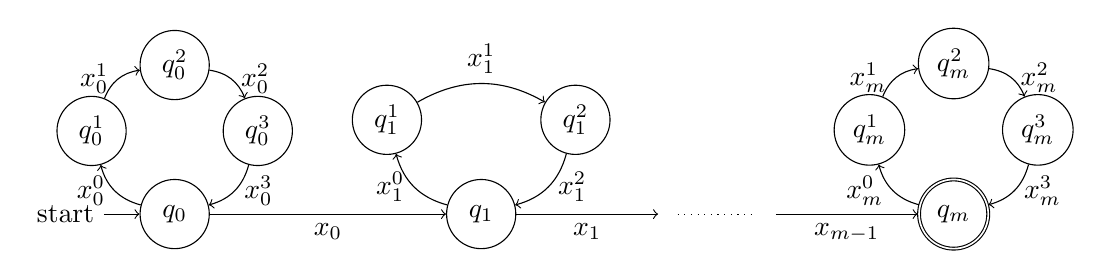
\begin{tikzpicture} 
		\node[state,initial] (q0)  {$q_0$};
		\node[state] (q1) [right = 3cm of q0] {$q_1$};
		\node (q2) [right = 1.8cm of q1]{};
		\node (q3) [right = 1cm of q2]{};
		\node[state,accepting] (qm) [right = 1.8cm of q3] {$q_m$};
		
		\node[state] (q01) [above left = 0.6cm of q0] {$q_0^1$};
		\node[state] (q02) [above = 1cm of q0] {$q_0^2$};
		\node[state] (q03) [above right = 0.6cm of q0] {$q_0^3$};

		\node[state] (q11) [above left = 0.8cm of q1] {$q_1^1$};
		\node[state] (q12) [above right = 0.8cm of q1] {$q_1^2$};

		\node[state] (qm1) [above left = 0.6cm of qm] {$q_m^1$};
		\node[state] (qm2) [above = 1cm of qm] {$q_m^2$};
		\node[state] (qm3) [above right = 0.6cm of qm] {$q_m^3$};

  		\draw[->] (q0) edge [bend left] node [left]{$x_0^0$} (q01) ;
  		\draw[->] (q01) edge [bend left] node [left]{$x_0^1$} (q02) ;
  		\draw[->] (q02) edge [bend left] node [right]{$x_0^2$} (q03) ;
  		\draw[->] (q03) edge [bend left] node [right]{$x_0^3$} (q0) ;
  		
  		\draw[->] (q0) edge node [below]{$x_0$} (q1) ;
  		\draw[->] (q1) edge node [below]{$x_1$} (q2) ;
  		\draw[dotted] (q2) edge (q3) ;
  		\draw[->] (q3) edge node [below]{$x_{m-1}$} (qm) ;

  		\draw[->] (qm) edge [bend left] node [left]{$x_m^0$} (qm1) ;
		\draw[->] (qm1) edge [bend left] node [left]{$x_m^1$} (qm2) ;
		\draw[->] (qm2) edge [bend left] node [right]{$x_m^2$} (qm3) ;
		\draw[->] (qm3) edge [bend left] node [right]{$x_m^3$} (qm) ;

  		\draw[->] (q1) edge [bend left] node [left]{$x_1^0$} (q11) ;
		\draw[->] (q11) edge [bend left] node [above]{$x_1^1$} (q12) ;
		\draw[->] (q12) edge [bend left] node [right]{$x_1^2$} (q1) ;
	\end{tikzpicture} 
	\caption{An example of a symbolic flat automaton}
\end{figure}

We say the FA $D=(Q,T',\Sigma_\epsilon,q_0,q_m)$ is an \emph{instance} of a SFA $S=(Q,T,\cvar_\epsilon,q_0,q_m)$, if there exists an interpretation $I: \cvar_\epsilon \rightarrow \Sigma_\epsilon$ satisfying $I(\epsilon)=\epsilon$ and $T'=\{(q,I(c),q')\mid (q,c,q')\in T\}$. We write $I(S)$ to denote the instance of $S$ wrt. $I$. The language of $S$ is defined as $L(S)= \cup\{L(D) \mid D \mbox{ is an instance of } S\}$. Notice that $L(S)$ is regular because every SFA has only finitely many instance and the finite union of regular languages are also regular.


For such kind of automata, the number of occurrence of each symbol in $\cvar$ uniquely characterize an accepting string. For example, if the string $x_1x_2x_1x_2$ is accepted, then all other strings with $\#(x_1)=\#(x_2)=2$ are not accepted. Moreover, from $\#(x_1)=\#(x_2)=2$, we can derive the accepted string $x_1x_2x_1x_2$ by exploring the automata structure. \todo{add Presburger constraints to allow more expressive power.}

\begin{lemma}
	Symbolic flat automata are closed under concatenation.
\end{lemma}





\todo{Mention NDD when talk about our practical bounded encoding for str2int}

\section{Handling Equality and Disequality Constraint} \label{section:eq}
Given an equality constraint $x_1\cdot x_2 \cdots x_n = x_{n+1}\cdot x_{n+2} \cdots x_m$, we restrict the domain of all variables to some SFA with disjunct alphabet and then connect the final state and initial state of two consecutive variables with an epsilon transition. 

For example, for the constraint $xy = yx$, if we restrict the domains of $x$ and $y$ to the SFA in Figure~\ref{fig:sfa} (a) and (b), respectively. We can then construct the SFA for $xy$ (Figure~\ref{fig:sfa} (c)) and $yx$ (Figure~\ref{fig:sfa} (d)).


\begin{figure}
	\tikzset{state/.style={circle,draw=blue!50,fill=blue!20,
			thick,inner sep=0pt,minimum size=6mm}, initial text=$ $}
		
 	\begin{minipage}[t]{0.15\textwidth} 
	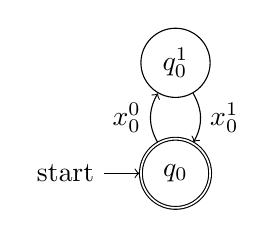
\begin{tikzpicture}
	\node[state,initial,accepting] (q0)  {$q_0$};
	
	\node[state] (q01) [above = 0.5cm of q0] {$q_0^1$};

	\draw[->] (q0) edge [bend left] node [left]{$x_0^0$} (q01) ;
	\draw[->] (q01) edge [bend left] node [right]{$x_0^1$} (q0) ;
	\end{tikzpicture} 
	
	\centering
	(a) $x$
	\end{minipage}
 	\begin{minipage}[t]{0.15\textwidth} 
	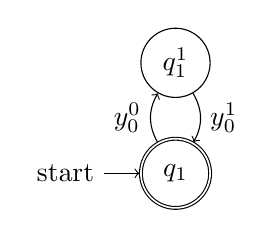
\begin{tikzpicture} 
	\node[state,initial,accepting] (q0)  {$q_1$};
	
	\node[state] (q01) [above = 0.5cm of q0] {$q_1^1$};
	
	\draw[->] (q0) edge [bend left] node [left]{$y_0^0$} (q01) ;
	\draw[->] (q01) edge [bend left] node [right]{$y_0^1$} (q0) ;
	\end{tikzpicture} 
	
	\centering
	(b) $y$
	\end{minipage}
	\ \ \ \ \ \ \ 
	\begin{minipage}[t]{0.28\textwidth}
	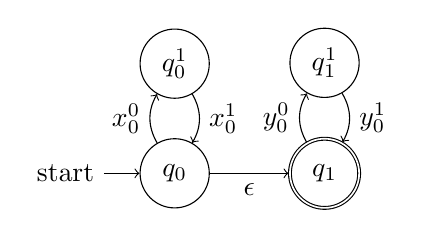
\begin{tikzpicture} 
	\node[state,initial] (q0)  {$q_0$};
	\node[state,accepting] (q1) [right = 1cm of q0] {$q_1$};
	
	\node[state] (q01) [above = 0.5cm of q0] {$q_0^1$};

	\draw[->] (q0) edge [bend left] node [left]{$x_0^0$} (q01) ;
	\draw[->] (q01) edge [bend left] node [right]{$x_0^1$} (q0) ;
	
	\node[state] (q11) [above = 0.5cm of q1] {$q_1^1$};
	
	\draw[->] (q1) edge [bend left] node [left]{$y_0^0$} (q11) ;
	\draw[->] (q11) edge [bend left] node [right]{$y_0^1$} (q1) ;
	\draw[->] (q0) edge  node [below]{$\epsilon$} (q1) ;
	\end{tikzpicture}
	
	\centering
	(c) $xy$
	\end{minipage}
	\begin{minipage}[t]{0.28\textwidth}
	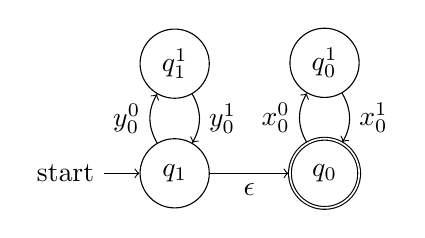
\begin{tikzpicture} 
	\node[state,accepting] (q0)  {$q_0$};
	\node[state,initial] (q1) [left = 1cm of q0] {$q_1$};
	
	\node[state] (q01) [above = 0.5cm of q0] {$q_0^1$};
	
	\draw[->] (q0) edge [bend left] node [left]{$x_0^0$} (q01) ;
	\draw[->] (q01) edge [bend left] node [right]{$x_0^1$} (q0) ;
	
	\node[state] (q11) [above = 0.5cm of q1] {$q_1^1$};
	
	\draw[->] (q1) edge [bend left] node [left]{$y_0^0$} (q11) ;
	\draw[->] (q11) edge [bend left] node [right]{$y_0^1$} (q1) ;
	\draw[->] (q1) edge  node [below]{$\epsilon$} (q0) ;
	\end{tikzpicture}
	
	\centering
	(d) $yx$
	\end{minipage}

	\caption{Symbolic flat automata of $x$, $y$, $xy$ and $yx$}
	\label{fig:sfa}
\end{figure}

Assume that $S_n=(Q,T,\cvar_\epsilon,q_i,q_f)$ is the SFA of $x_1\cdot x_2 \cdots x_n$ and $S_m=(Q',T',\cvar_\epsilon,q'_i,q'_f)$ is the SFA of $x_{n+1}\cdot x_{n+2} \cdots x_m$. Our next task is to find a model for $x_1\cdot x_2 \cdots x_n = x_{n+1}\cdot x_{n+2} \cdots x_m$ under the domain restriction specified by $S_n$ and $S_m$. 

This is equivalent to finding a common interpretation $I$ such that the languages of $I(S_n)$ and $I(S_m)$ are not disjoint. In order to find such an interpretation $I$, we first build a ``product'' automaton of $S_n$ and $S_m$ and then add some additional linear arithmetic constraints to force the two input automata sharing the same interpretation. 

Such product automaton uses $Q\times Q'$ as the set of states and $\cvar_\epsilon \times \cvar_\epsilon$ as the alphabet. If a transition $((q_1,q'_1), (x_1,x'_1),(q_2,q'_2))$ is taken, it means the character variable $x_1$ and $x'_1$ should be assigned the same value and this value leads $S_n$ from state $q_1$ to state $q_2$ and $S_m$ from $q'_1$ to $q'_2$.

More precisely, the product automaton $P$ is a tuple $(Q\times Q', T^2, \cvar_\epsilon \times \cvar_\epsilon, (q_i,q'_i),(q_f,q'_f))$, where the transition relation $T'$ is the minimal set satisfying the following.

\begin{itemize}
\item If $(q_1,x,q_2) \in T$, then for all $q'\in Q',((q_1,q'),(x,\epsilon),(q_2,q'))\in T^2$.
\item If $(q'_1,x,q'_2) \in T'$, then for all $q\in Q,((q,q'_1),(\epsilon,x),(q,q'_2))\in T^2$.
\item If $(q_1,x,q_2) \in T$ and $(q'_1,x',q'_2) \in T'$, then $((q_1,q'_1),(x,x'),(q_2,q'_2))\in T^2$.
\end{itemize}	
The first two cases correspond to the situation when the character variable $x$ is assigned $\epsilon$. In such cases, only one automaton changes its state.

The product automaton corresponds to $xy=yx$ can be found in Figure~\ref{}. 


\todo{This end of stable writing, the thing below is not consistent yet.}

\begin{figure}
	\tikzset{state/.style={circle,draw=blue!50,fill=blue!20,
			thick,inner sep=0pt,minimum size=6mm}, initial text=$ $}

	\begin{minipage}[t]{0.28\textwidth}
		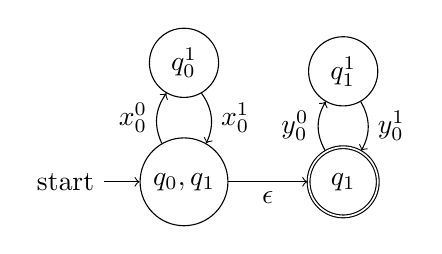
\begin{tikzpicture} 
		\node[state,initial] (q0)  {$q_0,q_1$};
		\node[state,accepting] (q1) [right = 1cm of q0] {$q_1$};
		
		\node[state] (q01) [above = 0.5cm of q0] {$q_0^1$};
		
		\draw[->] (q0) edge [bend left] node [left]{$x_0^0$} (q01) ;
		\draw[->] (q01) edge [bend left] node [right]{$x_0^1$} (q0) ;
		
		\node[state] (q11) [above = 0.5cm of q1] {$q_1^1$};
		
		\draw[->] (q1) edge [bend left] node [left]{$y_0^0$} (q11) ;
		\draw[->] (q11) edge [bend left] node [right]{$y_0^1$} (q1) ;
		\draw[->] (q0) edge  node [below]{$\epsilon$} (q1) ;
		\end{tikzpicture}
	\end{minipage}
	
	\caption{Product automaton of $xy=yx$}
	\label{fig:sfa}
\end{figure}




Recall that for flat automata, the number of occurrences of each symbol uniquely characterizes an accepting string. 






We first build a product automata $\mathcal{P}=(Q\times P, T, \cvar\times \cvar, (q_i,p_i), (q_f,p_f))$, where $((q,p),(x,y), (q',p'))\in T$ iff $(q,x,q')\in T_Q \wedge (p,y,p')\in T_P$. Then the following formula characterizes all models of the equality constraint $Parikh(\mathcal{P}) \wedge \#(x,y) > 0 \rightarrow \enc{x} = \enc{y}$.

In practice, building the product automata is an expensive operation. In practice, we consider SFA of special shape that allows more efficient translation from equality constraint to linear integer constraint.

We define $(p,q)$-SFA as a SFA consisting of $p$ simple loops of length $q$, connected by epsilon transitions. Formally, 

\todo{Maybe talk about the heuristic that we merge the list elements into one}





%%%%%%%%%%%%%%%%%%%%%%%%%%%%%%%%%%%%%%%%%%%%%%%%%%%%%%%%%%%%%%%%%%%%%%%%%%%%%%
\section{Handling String-Integer Conversion} \label{section:s2i}
%%%%%%%%%%%%%%%%%%%%%%%%%%%%%%%%%%%%%%%%%%%%%%%%%%%%%%%%%%%%%%%%%%%%%%%%%%%%%%
We begin the discussion with the conversion between bounded integers (e.g., 64-bits) and strings. Notice that even for bounded integer, the corresponding string can be of unbounded length. For example, the formula $\sti{x}=10 \wedge |x|=5$ is in fact satisfiable when $x=``00010"$. To handle the bounded integer case $y=\sti{x}$, we propose to restrict the domain of $x$ to a SFA of the form $(\{q_0,\ldots,q_k\},T,\cvar, q_0,q_k)$, where $k$ is the number of digits allowed in the bounded integer, $T = \{(q_0,x_0,q_0)\} \cup \{(q_i,x_{i+1},q_{i+1})\mid 0\leq i <k\}$, with additional numerical constraints $\enc{x_0}=\enc{\ch{0}}$ and $\wedge_{i\in [1,9]} \enc{\ch{0}}\leq \enc{x_i} \leq \enc{\ch{9}}$ to force the domain of the string to those corresponding to positive integers. Under this domain restriction, we obtain $y=\Sigma_{i\in [1,9]} 10^{k-i}\times (\enc{x_i}-\enc{\ch{0}})$.

\todo{Add an example: $\sti{x}=\sti{y} \wedge x= y\cdot y$. Do product construction informally here.}

This approach can be extended to unbounded string using more sophisticated pattern. For example, we can extend the bounded pattern that uses two loops, by changing the transition relation $T$ to $\{(q_0,x_0,q_0), (q_0,\epsilon,q_1), (q_k,x_1,q_1)\} \cup \{(q_i,x_{i+1},q_{i+1})\mid 0< i <k\}$. In this pattern, one can describe string that corresponds arbitrarily large integer. Taking the case $k=2$, $\enc{x_2}=\enc{\ch{3}}$, $\enc{x_1}=\enc{\ch{5}}$ as an example, any number in the form of $353535\ldots35$ can be expressed. Formally, the relation between $y$ and $x$ can be described in the following formula:
$$y= (10*(\enc{x_2}-\enc{\ch{0}})+(\enc{x_1}-\enc{\ch{0}}))\times \frac{100^{\#(x_1)}-1}{100-1}$$

where $\#(x_1)$ is the number of occurrence of $x_1$ in the corresponding symbolic string and is treated as a variable in this case. To solve the satisfiability of this formula, one need to solve an exponential constraint. From the results of POPL2019, this problem is decidable if ....




\end{document}
%%%%%%%%%%%%%%%%%%%%%%%%%%%%%%%%%%%%%%%%%%%%%%%%%%%%%%%%%%%%%%%%%%%%%%%%%%%%%%
